\chapter{Założenia i zasada działania}
Główne założenia oraz matematycznie aspekty pracy zostały opisane poniżej. Zilustrowano główne wzory na których bazuje projekt.
Moduł został zbudowany w oparciu o samochód Honda Civic VI z silnikiem D14A8 z roku 1998, jednak z łatwością można go dostosować, aby działał z innymi pojazdami.

\section{Przypadki użycia}
Końcowy użytkownik powinien móc odczytywać informacje, które po obliczeniach udostępnia mu mikrokontroler. Dodatkowo użytkownik ma mieć możliwość interakcji z modułem poprzez mikro przełącznik, tj. przełączanie karty menu, zmiana trybu podświetlenia oraz reset zapisanych danych. Powyższe przypadki użycia, w formie diagramu, zostały umieszczone na rys. \ref{fig:diagram}.

\begin{figure}[!htb]
\centering
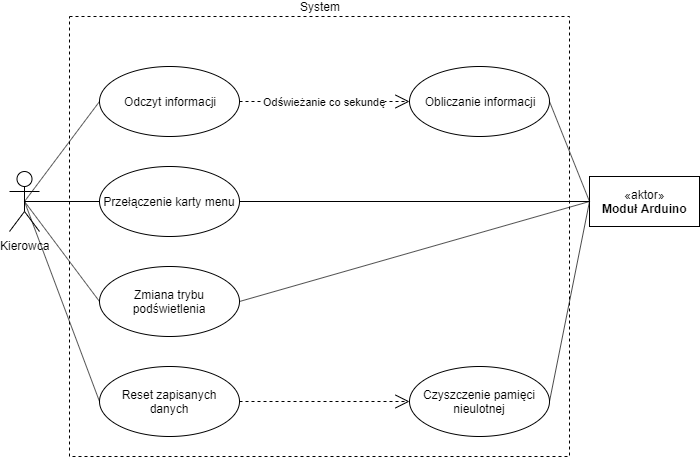
\includegraphics[width=1\linewidth]{Rysunki/diagram.png}
\caption{Diagram przypadków użycia}
\label{fig:diagram}
\end{figure}

\section{Obliczenia}
\par Informacje potrzebne do obliczenia aktualnego spalania to:
\begin{itemize}
\item{aktualna prędkość pojazdu}
\item{ilości wstrzykiwanego paliwa na jednostkę czasu}
\end{itemize}

\subsubsection{Obliczanie aktualnej prędkości pojazdu} \label{calc_speed}
VSS (Vehicle Speed Sensor) - jest to urządzenie, które przesyła dane do wskaźnika prędkości na desce rozdzielczej. Działa ono tak, iż wysyła określoną ilość impulsów co określony przejechany dystans. W przypadku pojazdu, na którym zbudowany został projekt jest to \textbf{4000 impulsów} co \textbf{jedną milę} (1609,344 metrów \cite{mila}).
\par Korzystając z podstawowego wzoru na prędkość \cite{fizyka}, można dojść do wniosku, iż jeżeli prędkość będzie odświeżana co sekundę oraz po odświeżeniu będzie resetowana ilość impulsów VSS to prędkość obliczona zostanie z wzoru (zobacz równanie (\ref{eq:speed})).

\begin{equation}\label{eq:speed}
V[km/h] = \frac{S[km]}{I} 3600 i
\end{equation}
gdzie:
\begin{description}
\item[S] długość jednostki dystansu, w przeliczeniu na kilometry, w której VSS wysyła sygnał
\item[I] to stała ilość impulsów VSS, co którą pojazd pokonuje określony dystans
\item[i] to liczba impulsów w tej sekundzie
\end{description}
W przypadku tego pojazdu wzór przedstawia się następująco (zobacz równanie (\ref{eq:speed2})).
\begin{equation}\label{eq:speed2}
V[km/h] = \frac{1.609344[km]}{4000} 3600i
\end{equation}

\subsubsection{Obliczanie spalania} \label{calc_consumption}
Koncepcja obliczania spalania polega na mierzeniu czasu otwarcia wtrysku, czyli czasu, w którym paliwo jest wstrzykiwane do komory spalania silnika. Jeśli znana jest stała wtryskiwacza, czyli parametr mówiący jaka ilość paliwa jest wtryskiwana w danym okresie czasu, można obliczyć aktualne spalanie samochodu.\\
Pojazd, na którym oparta jest ta praca posiada wtryski 190cc, co oznacza, że wtryskują one \textbf{190 ml paliwa na minutę}.

\subsubsection{Obliczanie spalania na godzinę}
Co jedną sekundę zostaje sprawdzone, przez jaki czas wtrysk wstrzykiwał paliwo. Mając już tę informację spalanie na godzinę zostaje wyliczone ze wzoru (\ref{eq:consumptionPerHour})

\begin{equation}\label{eq:consumptionPerHour}
C_{h}[L/h] = N\frac{I[ml]}{60}\frac{i[\mu s]}{1000000}\frac{3600}{1000}
\end{equation}
gdzie:
\begin{description}
\item[N] to ilość wtrysków w silniku
\item[I] to stała wtrysku
\item[i] to czas otwarcia wtrysku w danej sekundzie
\end{description}
\par Należy tutaj zaznaczyć, iż w projekcie pobierana jest informacja tylko z jednego wtrysku. Każdy wtrysk wstrzykuje za każdym razem tyle samo paliwa, więc ewentualny błąd przybliżenia do N wtrysków jest pomijalny.
\subsubsection{Obliczanie spalania na 100 km}
Bardziej przydatnym, z perspektywy odbiorcy, formatem aktualnego spalania jest spalanie zależne od aktualnej prędkości, czyli spalanie na 100 kilometrów. Zostaje ono obliczone ze wzoru (\ref{eq:consumptionPer100})

\begin{equation}\label{eq:consumptionPer100}
C_{100km}[L] = 100\frac{C_{h}[L/h]}{V[km/h]}
\end{equation}
gdzie:
\begin{description}
\item[C_{h}] to spalanie na godzinę
\item[V] to prędkość
\end{description}\\